\chapter{Sistema}
En este capitulo se introduce brevemente una serie de conceptos que fueron utilizados para la realización del presente proyecto integrador. No se pretende que el lector alcance una comprensión exhaustiva de los mismos, sino que tenga las herramientas necesarias para la correcta interpretación de los capítulos posteriores. De manera paralela se introducen los bloques básicos que formaran parte del sistema planteado.

\section{Sistemas Embebidos y Dispositivos Lógicos programables}

Un Sistema embebido es una combinación de hardware y software diseñado para realizar funciones dedicadas,generalmente en tiempo real. En algunos casos los sistemas embebidos no actúan de manera independiente y se encuentran integrados en un sistema o producto mayor.
En la actualidad el 98\% de los microprocesadores fabricados tienen como destino algún sistema embebido mientras que solo el 2\% se destina a microprocesadores de propósito general.

El campo de aplicación para los sistemas embebidos es muy variado, desde dispositivos portátiles como reproductores MP3 o teléfonos celulares, hasta sistemas de control en centrales nucleares.
No es posible caracterizar los componentes exactos de un sistema embebido ya que existen una gran cantidad de configuraciones posibles, pero dentro de los componentes fundamentales que se encuentran en la mayoría de los sistemas están:

\begin{itemize}
\item Microprocesador
\item Memoria RAM 
\item Periféricos para Captura de datos y de Comunicación.
\end{itemize}

\begin{figure}[h]
  \centering
	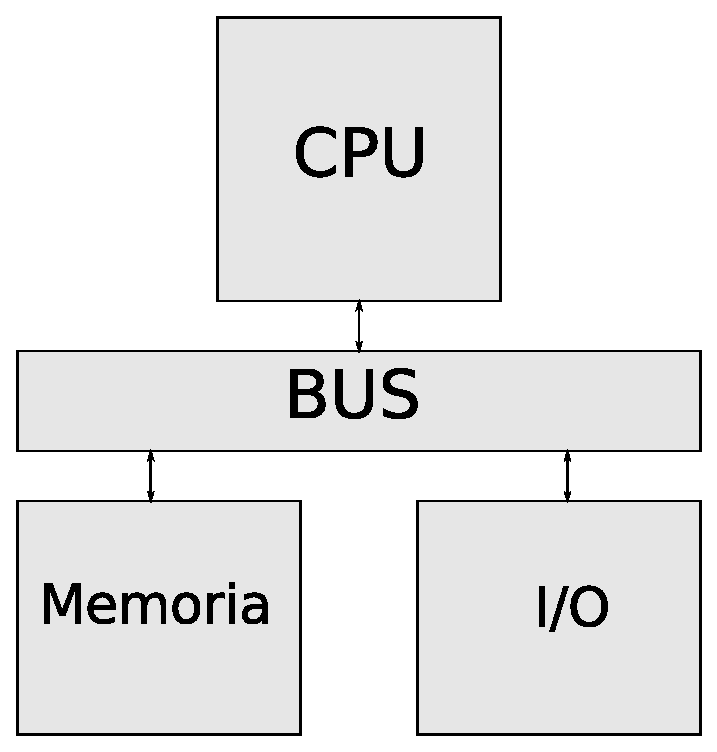
\includegraphics[width=0.70\textwidth]{2-sistema/graf/general.eps}
  \caption{Diseño preliminar}
  \label{figu:diseno}
\end{figure}

El sistema embebido que sera generado apartir de este proyecto no sera la excepción y contara al menos con los componentes anteriormente nombrados. En la Figura~\ref{figu:diseno} es posible ver el diseño preliminar del hardware de nuestro sistema.




\subsection{Dispositivos Lógicos Programables}
Los dispositivos lógicos pueden ser clasificados en dos categorías, fijos y programables. Los fijos son permanentes, están preparados para realizar una o una variedad especifica de funciones y una vez manufacturados no pueden ser modificados.
En cambio, los dispositivos lógicos programables, de ahora en adelante referenciados como PLDs, ofrecen como su nombre lo indica la posibilidad de ser reprogramados en cualquier momento con cualquier función lógica que el usuario requiere y que sea soportado por el dispositivo en cuestión.	

Existen dos grandes tipos de PLDs, FPGAs y CPLDs. Los CPLDs ofrecen una capacidad lógica pequeña, pero con unas características de temporización predecibles lo que los hace dispositivos ideales para aplicaciones de control y cualquier otra tarea de tiempo real. Además su consumo de potencia reducido y su bajo costo los posicionan muy bien en el campo de los dispositivos portátiles.
Por otro lado las FPGAs ofrecen una mayor densidad lógica y una mejor prerrománica. Actualmente es posible encontrar hasta 2 Millones de celdas lógicas en una FPGA comercial. Además estos dispositivos ofrece módulos embebidos como tranceptores, memoria o microprocesadores. Todo esto le permite a las FPGAs ser usadas en una amplia variedad de aplicaciones como procesamiento de datos, instrumentación, telecomunicaciones y procesamiento de señales.

\subsection{Sistemas embebidos en Logica Reprogramable}

ç



\section{Redes de Computadoras}

\subsection{Modelo OSI}

Es el modelo de red descriptivo creado por la Organización Internacional para la Estandarización en el año 1984. Sirve como marco de referencia para la definición de arquitecturas de interconexión de sistemas de comunicaciones.

\begin{figure}[h]
  \centering
	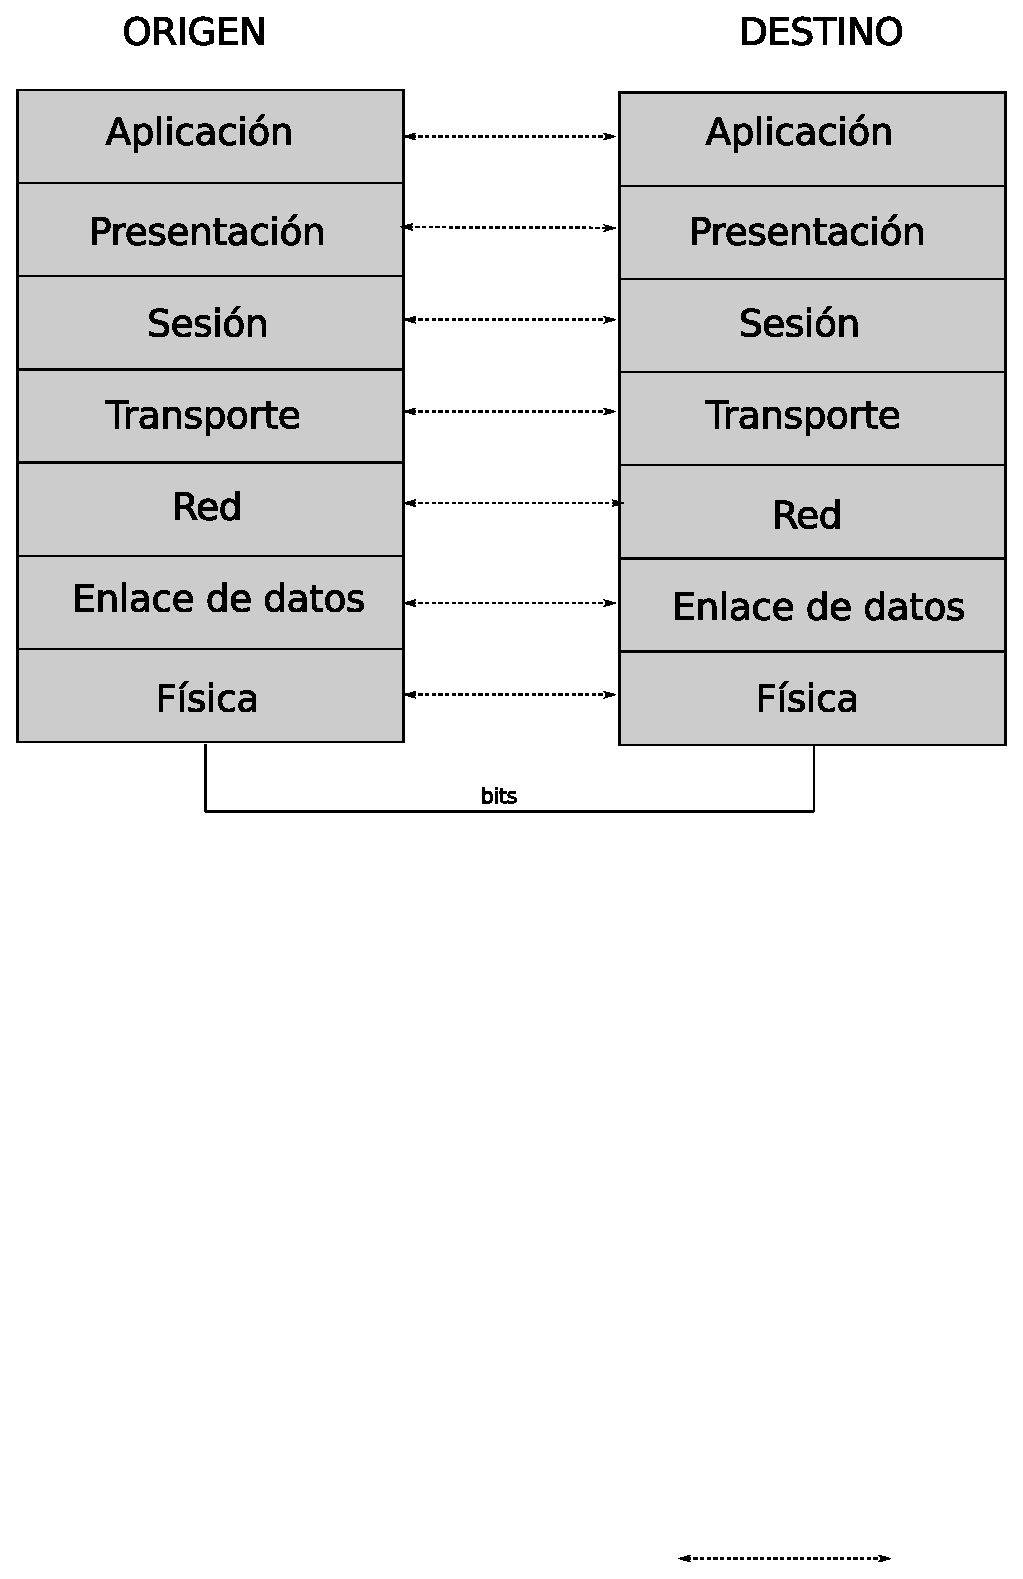
\includegraphics[width=0.80\textwidth]{2-sistema/graf/osi.eps}
  \caption{Modelo OSI}
  \label{fig:osi}
\end{figure}

Se basa en el concepto de \textit{capa}: Un conjunto de rutinas (y en algunos casos, hardware) que cumplen una serie de funciones determinadas. Cada capa ofrece servicios a las q se ubican por encima y hace uso de servicios ofrecidos por las de abajo. 



El modelo está conformado por las siguientes capas:

\begin{itemize}
	\item Aplicación: Representa el punto de acceso de las aplicaciones que hacen uso del esquema de transmisión de datos.
	\item Presentación: Relacionada con la representación de los datos.
	\item Sesión: se encarga de mantener y controlar el enlace establecido entre dos computadores que están transmitiendo datos.
	\item Transporte: encargada de efectuar el transporte de los datos (que se encuentran dentro del paquete) de la máquina origen a la de destino, independizándolo del tipo de red física que se esté utilizando.
	\item Red: Se encarga de identificar el enrutamiento existente entre una o más redes.
	\item Enlace de datos: se ocupa del direccionamiento físico, de la topología de la red, del acceso al medio, de la detección de errores, de la distribución ordenada de tramas y del control del flujo.
	\item Física: se encarga de las conexiones físicas de la computadora hacia la red, tanto en lo que se refiere al medio físico como a la forma en la que se transmite la información.
\end{itemize}

\subsubsection{Unidad de datos del protocolo}

Es un bloque de datos que cada capa utiliza para el intercambio de información con su par en el sistema destino. Suele denominarse PDU, por las siglas en inglés de \textit{Protocol Data Unit}.

\begin{figure}[h]
  \centering
	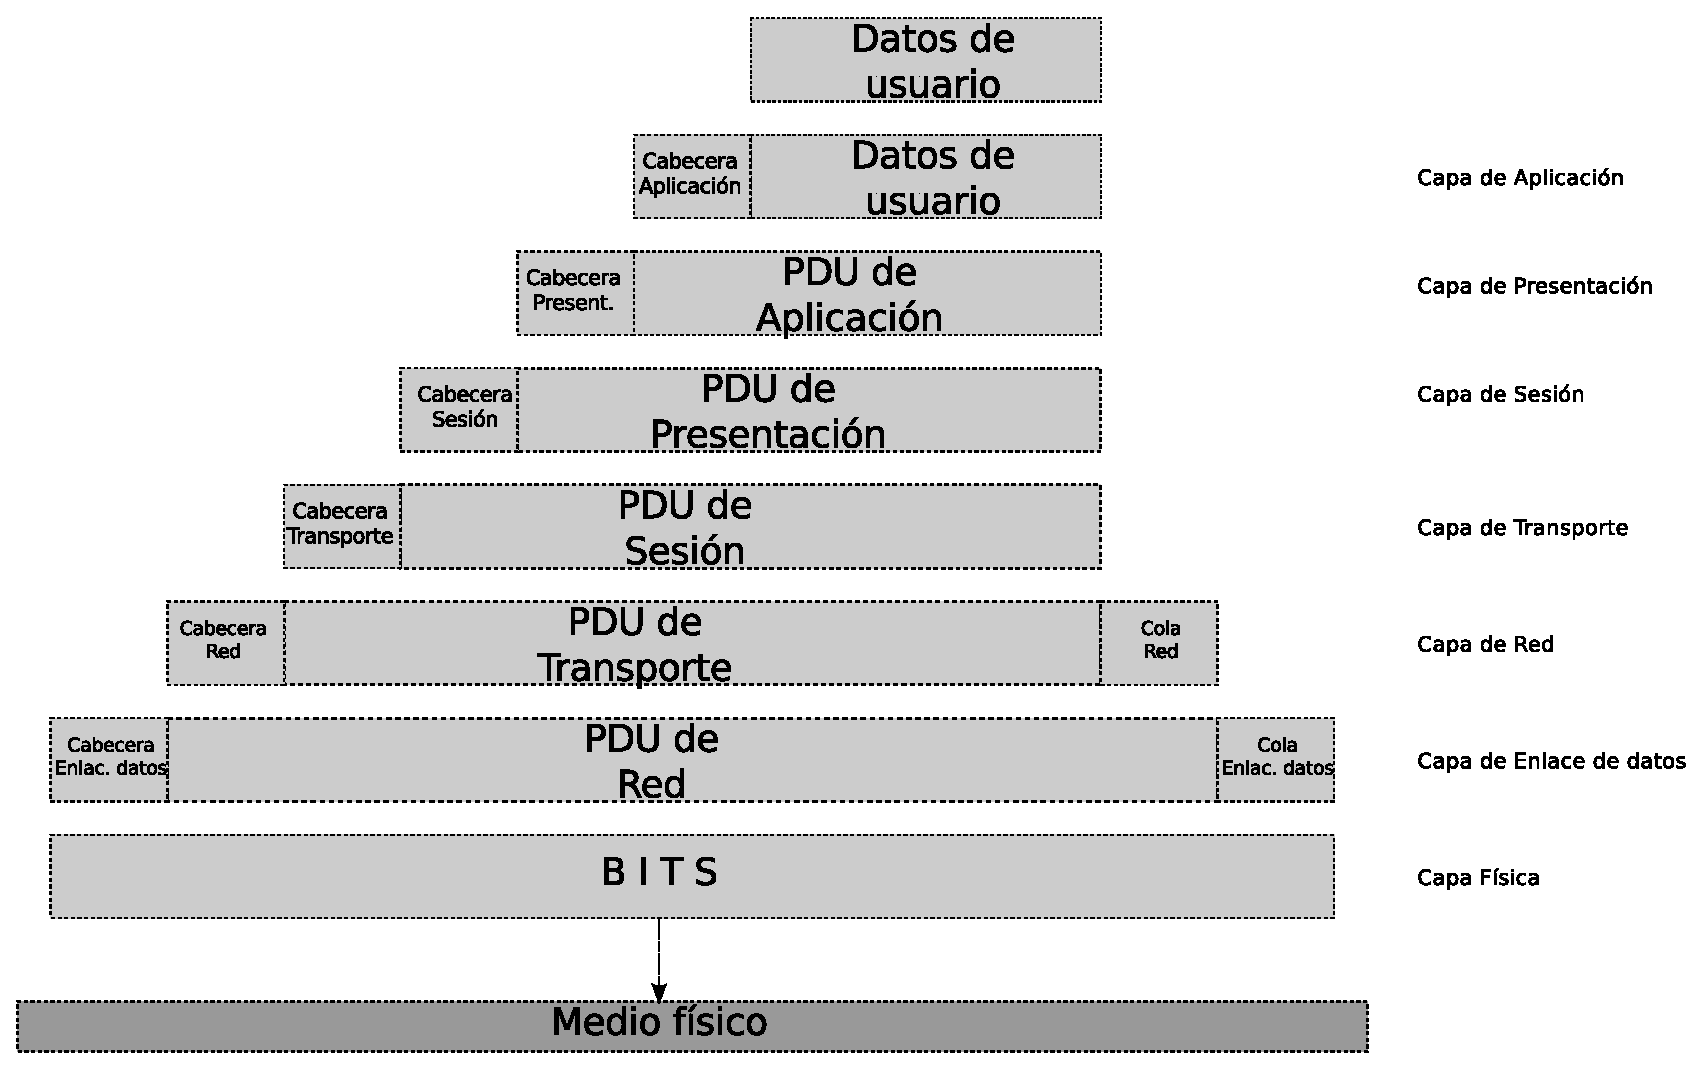
\includegraphics[width=0.90\textwidth]{2-sistema/graf/pdu.eps}
  \caption{PDUs en las distintas capas del modelo OSI}
  \label{fig:pdu}
\end{figure}

Cuando llega la información por parte del usuario, la capa de aplicación le agrega información de control y se conforma la PDU de dicha capa, la cual es transferida a la siguiente, que va a hacer lo mismo. De esta manera, cada capa agrega información a la PDU recibida de la anterior y transfiere la PDU resultante hacia la de abajo. Esto se repite hasta llegar al nivel físico, en el cual la información se transmite desde el sistema origen hacia el sistema destino en forma de bits.

Una vez que los datos han llegado a destino, comienza el proceso inverso. Los bits en capa física son transferidos a la capa de enlace de datos, la cual los delimita conformando tramas (PDUs de dicha capa). En base a la información de control, cada capa va transfiriendo su PDU hacia arriba, hasta que los datos llegan a la aplicación de destino. Se dice que la comunicación entre capas pares es transparente, ya que cada una de ellas no es consciente de los detalles de la implementación de las capas inferiores, tanto en el sistema origen como en el sistema destino. La figura ~\ref{fig:osi} muestra este concepto.

\subsection{TCP/IP}

Es un conjunto de protocolos de red en los que se basa Internet y que permiten la transmisión de datos entre computadoras. Se le denomina simplemente TCP/IP, en referencia a los dos protocolos más importantes que la componen: Protocolo de Control de Transmisión (TCP) y Protocolo de Internet (IP).

\subsubsection{Relación con el modelo OSI}

TCP/IP puede describirse como un modelo de capas al igual que OSI. Sin embargo, éste último es más bien una abstracción teórica, que sirve como referencia, mientras que TCP/IP es una implementación práctica que cuenta con 5 capas en vez de 8.





\subsection{Ethernet}

Ethernet es un estándar de transmisión de datos para redes de área local. El mismo define las características del cableado y señalización en capa física, así como también el formato de trama en capa de enlace de datos. 

\subsubsection{Formato de trama}

\begin{itemize}
	\item SOP (Start of packet): Indica el comienzo de un paquete.
	\item Source Address: Indica la dirección MAC de origen.
	\item Destination Address: Indica la dirección de destino.
	\item Ethertype / Length: Indica el tipo de trama o el tamaño de la misma, dependiendo de la versión de Ethernet.
	\item EOP (End of packet): Indica el final de un paquete.
\end{itemize}





\subsection{Búsqueda del prefijo más largo}

(... pendiente ...)


*-*-* Esto queda como reserva de datos que despues vmaos a usar****

Uno de los mayores cuellos de botella en los routers lo constituye el cómputo de del prefijo más largo para cada paquete entrante.

Implementar ciertos esquemas de clasificacion en hardware se ve limitado principalmente debido a 2 factores: La cantidad de memoria requerida y lla complejidad creciente de los mismos.

En tanto crece el trafico en las redes se ve la necesidad de implementar esquemas mas complejos de clasificacion.

Dichos esquemas tienen una implementación más sencilla en software. Dichas implementaciones estan ampliamente difundidas en la web.
Esto hace innecesario tener que “adaptarlas” a un HDL. El paso es trivial (corregir esta redaccion)

\section{FPGA}
Son dispositivos lógicos programables cuya lógica interna puede ser reconfigurada. Esta característica permite implementar un diseño propio, con la posibilidad de efectuar la cantidad necesaria de pruebas hasta llegar a los resultados deseados. Se puede instanciar componentes usando la lógica interna (ej microprocesadores, PLL, Memorias,etc).

\section{Sistemas embebidos}
Aunque se pone mucho foco en el  diseño de los procesadores de proposito general en la realidad estos solo representan solo una pequeña proporcion de los procesadores efectivamente producidos cada año.  Existe una especial motivacion en la industria por los denominados “Procesadores Heterogeneos” que integran sistemas dedicados con procesadores de proposito general.

(acá se podría poner algunas generalidades sobre Ethernet e IP)

(tambien se podria agregar algo del problema del prefijo más largo)


El sistema implementado en el presente trabajo consta de un microprocesador NIOS2/f interconectado mediante un bus Avalon-MM a 5 componentes: 
\begin{itemize}
\item PLL
\item JTAG UART
\item Iterfaz con SDRAM
\item Timer
\item Módulo extractor de cabeceras
\end{itemize}


\begin{figure}[h]
  \centering
	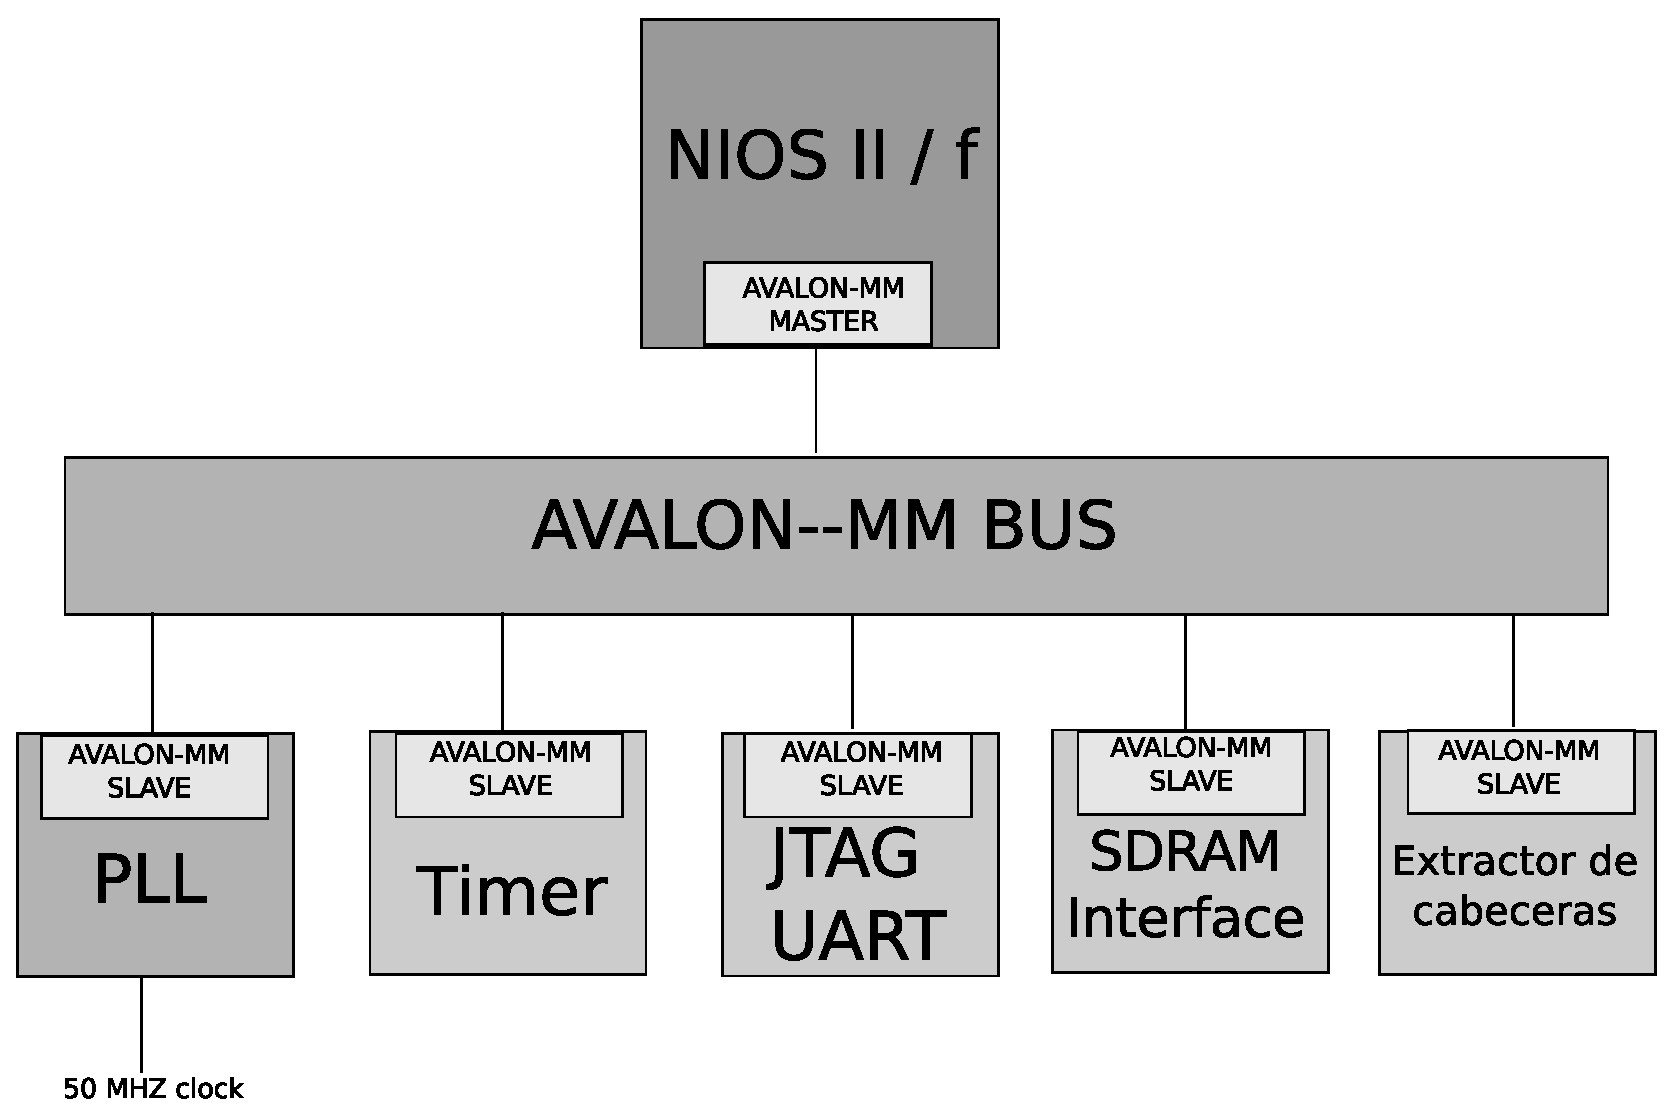
\includegraphics[width=0.80\textwidth]{2-sistema/graf/sistema.eps}
  \caption{Sistema}
  \label{fig}
\end{figure}

A su vez, éste último está conformado por un generador de paquetes Ethernet conectado a una FIFO. Esta está a su vez conectada a un modulo denominado delay buffer, que está conectado al modulo uplink y al write output.. Uplink a su vez está conectado también a write output.

\begin{figure}[h]
  \centering
	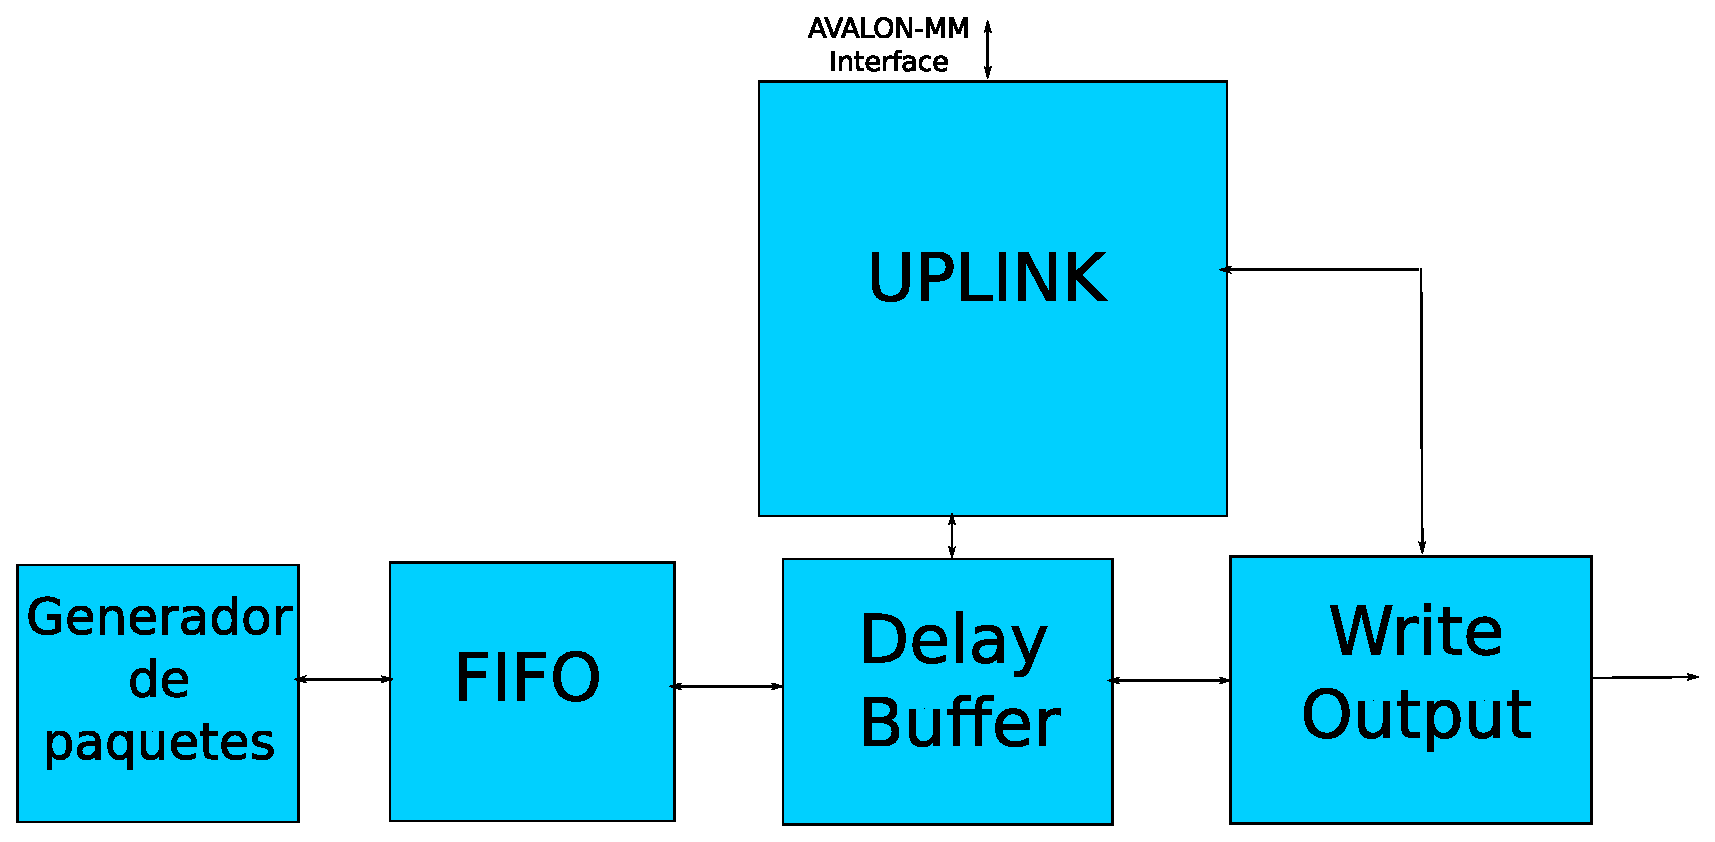
\includegraphics[width=0.80\textwidth]{2-sistema/graf/extractor.eps}
  \caption{Extractor de cabeceras}
  \label{fig}
\end{figure}

Sobre el hardware descrito anteriormente se ejecuta un software de clasificacion de paquetes, que se encuentra almacenado en una memoria RAM.



%\section{Distribucion Lineal}
